\section{Convex functions}
\subsection{Extended-valued functions}
\begin{definition}[Extended-valued function]
    A function $f: \R^n \longrightarrow \R$ is \emph{extended-valued} if its domain is $\R^n$ and its range is $\bar{\R} := \R \cup \{+\infty\}$.
\end{definition}

\begin{example}[Indicator function]
    We consider the indicator function of interval $[a, b]$:
    \begin{equation*}
        \ind_{[a,b]}(x) := \begin{cases*}
            0 & if $x\in[a,b]$ \\
            +\infty & otherwise
        \end{cases*}
    \end{equation*}
    \begin{figure}[H]
        \centering
        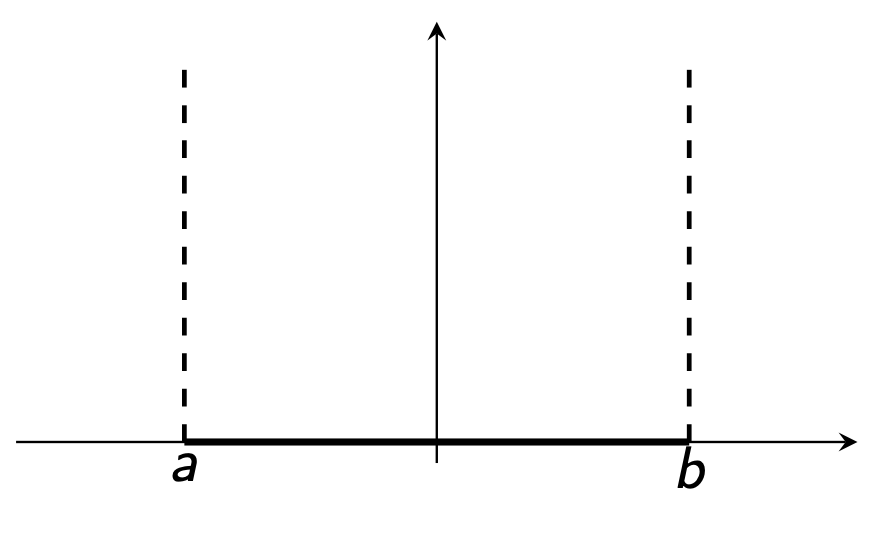
\includegraphics[width=.4\textwidth]{convex-functions/indicator.png}
    \end{figure}
\end{example}

\begin{definition}[Effective domain]
    The \emph{effective domain} of $f:\R^n\longrightarrow\bar{\R}$ is the set of points where $f$ is finite:
    \begin{equation*}
        \dom f := \set{x\in\R^n}{f(x)<+\infty}
    \end{equation*}
\end{definition}

A function is said to be \emph{proper} if its effective domain is non-empty: $\dom f \neq \emptyset$.

\begin{definition}[Epigraph]
    The \emph{epigraph} of a function $f:\R^n\longrightarrow\bar{\R}$ is the set of points lying above the graph of $f$:
    \begin{equation*}
        \epi f := \set{(x, t)\in\R^n\times\R}{f(x)\leq t}
    \end{equation*}
\end{definition}